\chapter{Timeline, Reviews and Work Division}\label{ch:timeline}

\section{From proposal to final results}
\begin{figure}[H]\centering
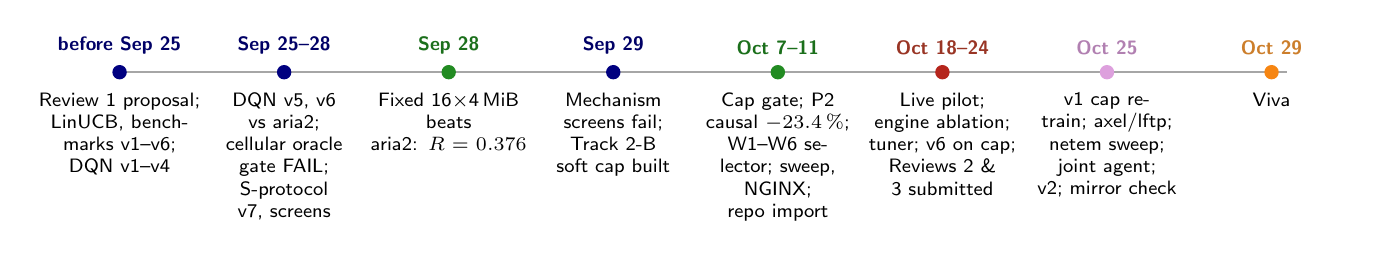
\begin{tikzpicture}[x=0.95cm,y=1cm,font=\sffamily\scriptsize]
\draw[thick,gray!70] (0,0) -- (15.6,0);
\foreach \x/\d/\t/\c in {
 0.0/{before Sep 25}/{Review 1 proposal;\\LinUCB, benchmarks v1--v6;\\DQN v1--v4}/NavyBlue,
 2.2/{Sep 25--28}/{DQN v5, v6 vs aria2;\\cellular oracle gate FAIL;\\S-protocol v7, screens}/NavyBlue,
 4.4/{Sep 28}/{Fixed 16$\times$4\,MiB beats\\aria2: $R=0.376$}/ForestGreen,
 6.6/{Sep 29}/{Mechanism screens fail;\\Track 2-B soft cap built}/NavyBlue,
 8.8/{Oct 7--11}/{Cap gate; P2 causal $-23.4\,\%$;\\W1--W6 selector; sweep,\\NGINX; repo import}/ForestGreen,
 11.0/{Oct 18--24}/{Live pilot; engine ablation;\\tuner; v6 on cap;\\Reviews 2 \& 3 submitted}/BrickRed,
 13.2/{Oct 25}/{v1 cap retrain; axel/lftp;\\netem sweep; joint agent;\\v2; mirror check}/Plum,
 15.4/{Oct 29}/{Viva}/BurntOrange}{
  \fill[\c] (\x,0) circle (2.6pt);
  \node[above=3pt,text=\c!80!black,font=\sffamily\scriptsize\bfseries] at (\x,0) {\d};
  \node[below=4pt,align=center,text width=2.1cm] at (\x,0) {\t};
}
\end{tikzpicture}
\caption{Project timeline. Dates from \code{docs/PROJECT\_CONTEXT.md} and the git log (which begins 2026-10-11); the Review~1 date is not recorded in the repository.}\label{fig:timeline}
\end{figure}

\begin{table}[H]\centering\small
\caption{Dated milestones}\label{tab:milestones}
\begin{tabularx}{\linewidth}{@{}P{2.6cm}L@{}}
\toprule
\textbf{Date (2026)} & \textbf{Milestone}\\
\midrule
not recorded & Review~1 proposal (``Assessment 8'', a seven-week plan): adaptive HTTP download manager with joint $N$/$S$ adaptation using RL. Early LinUCB calibration and benchmarks v1--v6; DQN candidates v1--v4.\\
Sep 25 & Mobile traces retrieved; seed date for the v5/v6 evaluations; DQN v5 and v6 head-to-heads, long-duration diagnostic, environment designs L2--L4, live probes T1/T2, mobile chain M1--M3.\\
Sep 26--27 & Mahimahi replay diagnostics; Stage 0 epoch pilot; oracle preregistrations v2--v4; tau (switch-cost) campaign.\\
Sep 28 & Cellular oracle gate \textbf{fails} (LCB $-0.26$\,\%); S-protocol v7 frozen and Stage 0S feasibility GO; S and N mechanism screens fail; \textbf{fixed $16\times4$\,MiB beats aria2 by 62.4\,\%} (30 pairs).\\
Sep 29 & Phase-pacing, queueing and correlated-loss screens fail; Track~1 (heuristic joint N+S on D2: 2.32$\times$ slower than fixed); Track~2 pre-screen stopped; Track~2-B soft cap implemented; team status note.\\
Oct 7 & Track~2-B live fixed-grid gate: fails one of six checks (S-margin 3.74\,\% vs 5\,\%).\\
Oct 8--9 & P1 selector and P2 within-download controller ($R=0.766$, $-23.4\,\%$); S-only ablation; W1--W6 design and live comparison (selector 0.999).\\
Oct 11 & Repository import commit; verification audit; pacing sweep and NGINX check; claims checker 113 of 113.\\
Oct 12 & \code{paper-rc1}; model-based controller attempt stopped at its gate (0 of 6).\\
Oct 18--20 & Live-internet pilot on four public mirrors (protocol frozen Oct 18).\\
Oct 24 & Pilot analysed; study audit finds the engine flaws; split ablation (230 runs); online tuner (64); frozen v6 on the capped server (50); \textbf{Review~2 and Review~3 submitted}.\\
Oct 25 & Cap-trained DQN v1 (Stages A--D); axel/lftp baselines (80); delay$\times$loss sweep (108); joint N+S agent (150 + 40); DQN v2 (24 + 8 + 64 + 160); real-mirror check (M1 aborted, M2 60 of 60); paper and checker to 220 of 220.\\
Oct 29 & Viva (Thursday).\\
\bottomrule
\end{tabularx}
\end{table}

\section{What each review covered}
\subsection{Review 1: the proposal}
Title: \emph{Adaptive HTTP File Download Manager with Joint Concurrency and Chunk-Size Adaptation using Reinforcement Learning}. Its own words matter in the viva: it positioned the project ``as an engineering and experimental contribution rather than a claim of inventing adaptive segmented downloading'', and promised to \emph{investigate} ``whether jointly selecting $(N, S)$ provides a measurable advantage''. It explicitly said: ``The evaluation does not depend exclusively on successful RL convergence''.

Proposed components: Network Monitor, Context Builder, Adaptive Decision Engine/Policy, Concurrency Manager, Range Manager, Request Scheduler, HTTP Fetcher + Writer, Test Server/Network Emulator. Seven-week plan: (1) core stabilization and test environment; (2) network monitor and policy foundation; (3) runtime adaptive control; (4) heuristics and LinUCB; (5) RL integration; (6) experiments; (7) analysis, paper, demo. Expected comparisons: fixed vs heuristic; $N$-only vs $S$-only vs joint; LinUCB vs RL; aria2 and IDM ``where reproducible experimental access is available''; stable vs variable bandwidth, latency/loss, throttling, background traffic, combined conditions.

\subsection{Review 2: progress (submitted 24 Oct)}
System architecture, detailed design, algorithm, UML and DFDs, modules, prototype, the first benchmark (62.4\,\% vs aria2), the pacing sweep and NGINX check, 549 test functions, and the individual-contribution table.

\subsection{Review 3: final report (submitted 24 Oct)}
Complete system, straggler splitting, online tuner, live demo, test results, goodput and reliability, the engine ablation, ``does adaptation help'', adaptation speed, the tuner, other searches, real networks (live pilot, cellular traces), learned policies incl.\ the frozen v6 on the capped server, limitations, comparison with aria2, objectives and deviations, innovation, future work, and the publication plan (IEEE Access).

\subsection{After the reviews (25 Oct): all planned experiments complete}
Review~3's ``future enhancement'' list had seven items. The first three were done, plus two extra studies; the rest (broader live study, HTTP/2 and multiple sources, splitting by default with a stall-based timeout, PPO and IDM) remain future work:
\begin{enumerate}
\item \textbf{An agent trained for the capped server} $\rightarrow$ cap-trained DQN v1 (\code{rl\_cap\_train}), then broader-trained v2 (\code{rl\_cap\_train\_v2}).
\item \textbf{More baselines in the same testbed} $\rightarrow$ axel and lftp (\code{baselines\_ext}); wget2 shown unable to download one file in parallel.
\item \textbf{Joint learning on harder environments} $\rightarrow$ joint N + range-size agent with a live-rate control server (\code{rl\_joint}).
\item \textbf{Extra: delay and loss sweep} $\rightarrow$ $3\times3$ grid (\code{netem\_sweep}).
\item \textbf{Extra: adaptive agents on real servers} $\rightarrow$ no-harm check on three mirrors (\code{live\_mirror\_check}).
\end{enumerate}

\section{Objectives and deviations}
\begin{table}[H]\centering\small
\caption{Review~1 objectives and outcomes (updated with the post-review studies)}\label{tab:objectives}
\begin{tabularx}{\linewidth}{@{}P{5.0cm}P{1.7cm}L@{}}
\toprule
\textbf{Objective (Review 1)} & \textbf{Status} & \textbf{Outcome}\\
\midrule
Correct segmented downloader, one range per request & Achieved & Byte-identical output; probe and SHA-256 check in the CLI\\
Controlled test server with throttling and faults & Achieved & Pacing, soft cap, live-rate mode, fault injection\\
Network monitor over rolling windows & Achieved & Metrics + rolling-window state: per-request and aggregate throughput, TTFB, failures, retries\\
Policy interface: fixed, heuristic, LinUCB, RL & Achieved & One interface runs all of them\\
Joint adaptation of $N$ and $S$ & Achieved & Rule-based, causal, LinUCB, DQN v2/v3, and the joint N+S agent; none beat the best fixed setting\\
Evaluate under stable, variable, lossy, throttled, background-traffic conditions & Achieved & Rate schedules; netem (incl.\ a $3\times3$ delay--loss grid); cellular traces; live internet; capped servers; \code{iperf3} background traffic\\
Compare on time, goodput, reliability, adaptation speed & Achieved & All four reported\\
$N$-only, $S$-only, joint ablation & Achieved & CAP8: $N$-only 0.808, joint 0.766, $S$-only 1.070 of fixed\\
LinUCB vs RL & Partly & Both evaluated, not in one predeclared head-to-head\\
aria2 and IDM & aria2 yes; IDM no & aria2 throughout; axel, lftp added; IDM not reproducible on Linux\\
\bottomrule
\end{tabularx}
\end{table}

\begin{table}[H]\centering\small
\caption{Deviations from the Review~1 plan and why}\label{tab:deviations}
\begin{tabularx}{\linewidth}{@{}P{4.4cm}L@{}}
\toprule
\textbf{Deviation} & \textbf{Reason}\\
\midrule
Framing: from ``build an RL download manager'' to ``when does adaptation help?'' & Early results showed well-chosen fixed settings near-optimal; the system, scope and policies stayed as planned.\\
Final DQN learns $N$ only ($S=1$\,MiB) & v2 fragmented ranges into 32--128\,KiB pieces; v3's simulator rewarded large ranges the server did not. (The later joint agent revisited $S$ and lost.)\\
No PPO or hybrid agent & After LinUCB locked onto one action, Double DQN was carried through to live evaluation; PPO is future work.\\
Decisions after each completed request, not every fixed interval $T$ & The live runner decides per completed attempt; the simulator was aligned after a v5 mismatch.\\
In-flight ranges were not split (until the audit) & Kept for correctness; the ablation showed this was the main reason aria2 led under the cap, so splitting was added as an opt-in.\\
No resume from disk & Outside the evaluated scope.\\
Cobra, slog, gRPC, \code{x/time/rate} not used & The standard library sufficed; DQN runs inside Go from exported weights, so no RPC; the server needed its own rate model.\\
FastBioDL evaluated as a re-implementation & Its idea was re-implemented and tested under a frozen protocol.\\
\bottomrule
\end{tabularx}
\end{table}

\section{Work division}\label{sec:work}
The work division below is the ``Individual Contribution'' table from the submitted Review~2 report, which states that ``responsibilities follow the division of work set out in the Review~1 proposal''. (The Review~1 proposal file in the repository has no per-member table, so Review~2's table is the record.) Each member's subsection then lists the parts of this handbook that fall in that area, as a study guide: \emph{these are the topics an examiner is most likely to ask that member about}.

\begin{table}[H]\centering
\caption{Team members and contributions (from Review~2)}\label{tab:team}
\begin{tabularx}{\linewidth}{@{}p{3.2cm}p{2.1cm}L@{}}
\toprule
\textbf{Member} & \textbf{Reg.\ no.} & \textbf{Contribution}\\
\midrule
\MemberA & \RegA & Downloader architecture and core implementation; adaptive concurrency and range management; test server and Linux network experiments; system integration and validation\\
\MemberB & \RegB & Downloader development and testing of assigned components; monitoring and experiment automation; baseline and heuristic evaluation\\
\MemberC & \RegC & LinUCB; RL state, action and reward design; Python/PyTorch models; integration of the learned policy with the Go downloader; ML/RL evaluation\\
\bottomrule
\end{tabularx}
\end{table}

\subsection{\MemberA\ (\RegA): architecture, core engine, server and network experiments}
\textbf{Stated work:} downloader architecture and core implementation; adaptive concurrency and range management; test server and Linux network experiments; system integration and validation.

\textbf{Be ready to explain:}
\begin{itemize}
\item The architecture and every engine component (Table~\ref{tab:components}); the five invariants; half-open ranges and the single conversion point; retries with unchanged bounds; why lowering $N$ never cancels a request.
\item The worker loop, the policy runner's lock, and the controllers.
\item Straggler splitting ($m = s+b+\lfloor r/2\rfloor$, the 2\,MiB minimum) and the request deadline; the engine ablation and why it changed the conclusion (Chapter~\ref{ch:cap}).
\item The paced server's three rules, the request-start rate rule, the soft cap formula (\ref{eq:cap}), the live-rate mode, fault injection.
\item netem (40\,ms each way = 80\,ms RTT, 0.4\,\% loss), the delay--loss sweep, Mahimahi replay, the live-pilot runner and mirror etiquette.
\item The D2 mechanism (why 112 of our 128 requests start after the speed-up), the granularity control (0.862), the constant-rate controls.
\item Validation: SHA-256 checks, the test suite, race detector, the claims checker.
\item The demo steps 1 and 2 (Chapter~\ref{ch:presentation}).
\end{itemize}

\subsection{\MemberB\ (\RegB): components, monitoring, automation, baselines and heuristics}
\textbf{Stated work:} downloader development and testing of assigned components; monitoring and experiment automation; baseline and heuristic evaluation.

\textbf{Be ready to explain:}
\begin{itemize}
\item Metrics and monitoring: per-attempt records, per-request vs aggregate throughput, TTFB, rolling windows, the run record fields (Chapter~\ref{ch:system}).
\item Test types and representative test cases; failure-handling tests (\code{200} instead of \code{206}, short bodies, wrong \code{Content-Range}).
\item Experiment automation: arms, blocks, seeded order, fresh state per run, validity rules, netem status recording, the harness programs.
\item Baselines: aria2 flags and how they were chosen; axel, lftp, curl, NGINX; why not wget2 and IDM (Chapter~\ref{ch:aria2}).
\item Heuristic controllers: the throughput rule, the causal drop rule, the workload selector, the online tuner; their results and adaptation speed (Chapter~\ref{ch:cap}).
\item The statistics: geometric mean, bootstrap, $t$-interval, verdicts, workload-level intervals (Chapter~\ref{ch:method}).
\item The live-pilot and mirror-check results and how the link gate worked (Chapter~\ref{ch:real}).
\item Demo step 3: tests and the claims checker.
\end{itemize}

\subsection{\MemberC\ (\RegC): LinUCB, RL design, models and learned-policy evaluation}
\textbf{Stated work:} LinUCB; RL state, action and reward design; Python/PyTorch models; integration of the learned policy with the Go downloader; ML/RL evaluation.

\textbf{Be ready to explain:}
\begin{itemize}
\item LinUCB: features, actions, reward, the UCB formula, and why it locked onto one action (Chapter~\ref{ch:learned}).
\item DQN and Double DQN (equations in Chapter~\ref{ch:background}); the 13 state features; actions; reward $r_t=-\Delta t$; hyperparameters; network $13\to64\to64\to3$.
\item The DQN version history v1--v6 and why each changed; why $S$ was removed from the action at v4.
\item The simulators, what the v6 simulator got wrong, calibration from request logs, blind parity checks, Go inference and parity tests.
\item The cap-trained v1, the joint agent, and v2: training distributions, seed selection on validation only, held-out scenario design and headroom, results, the drop-rule comparison (Chapter~\ref{ch:learned}).
\item The oracle and headroom gates, and the argument ``the opportunity, not the learner, was the bottleneck'' (Chapter~\ref{ch:synthesis}).
\item The model-based attempt and the L4 simulator-only headroom.
\end{itemize}

\begin{vivatip}
Everyone should be able to give the one-page story (Chapter~\ref{ch:overview}) and the novelty statement (Section~\ref{sec:novelty}). If a question goes to another member's area, answer the headline and say ``\emph{[name] can give the detail}''. That shows teamwork and is better than guessing.
\end{vivatip}
